% Face Masks Market Analysis Presentation
% Created for exploratory data analysis project

\documentclass[aspectratio=169]{beamer}

% Packages
\usepackage{fontspec}
\usepackage{graphicx}
\usepackage{booktabs}
\usepackage{tabularx}
\usepackage{xcolor}
\usepackage{ragged2e}
\usepackage{hyperref}
\usepackage{caption}
\usepackage{float}

% Theme settings
\usetheme{Singapore}
\usecolortheme{orchid}
\setbeamertemplate{navigation symbols}{}
\setbeamertemplate{caption}[numbered]
\setbeamerfont{frametitle}{size=\large,series=\bfseries}
\setbeamercolor{frametitle}{fg=purple!70!black}
\setbeamercolor{title}{fg=purple!80!black}

% Title information
\title{Face Masks Market Analysis}
\subtitle{Insights for Manufacturers \& Marketers}
\author{Sayan Ghosh}
\date{\today}
\institute{Indian Institute of Technology Madras}

\begin{document}

\begin{frame}
\titlepage
\end{frame}

\begin{frame}
\frametitle{Contents}
\tableofcontents
\end{frame}

\section{Introduction}

\begin{frame}
\frametitle{Project Overview}
\begin{itemize}
    \item \textbf{Objective:} Provide insights to a manufacturer of personal care products regarding the face mask market
    \item \textbf{Data Sources:}
    \begin{itemize}
        \item Product listings data (\(n=27\) products)
        \item Customer review data (\(n=3,849\) reviews)
    \end{itemize}
    \item \textbf{Analysis Focus:}
    \begin{itemize}
        \item Market segmentation and competitive landscape
        \item Customer preferences and sentiments
        \item Price positioning and value perception
        \item Opportunities for product development
    \end{itemize}
\end{itemize}
\end{frame}

\section{Market Overview}

\begin{frame}
\frametitle{Face Mask Types in the Market}
\begin{columns}
\column{0.5\textwidth}
\begin{itemize}
    \item The market contains several distinct mask types
    \item Disposable masks dominate the online marketplace
    \item Respirators (KN95, N95) represent a significant segment
    \item Specialized masks (copper, nano-tech) are emerging niches
\end{itemize}
\column{0.5\textwidth}
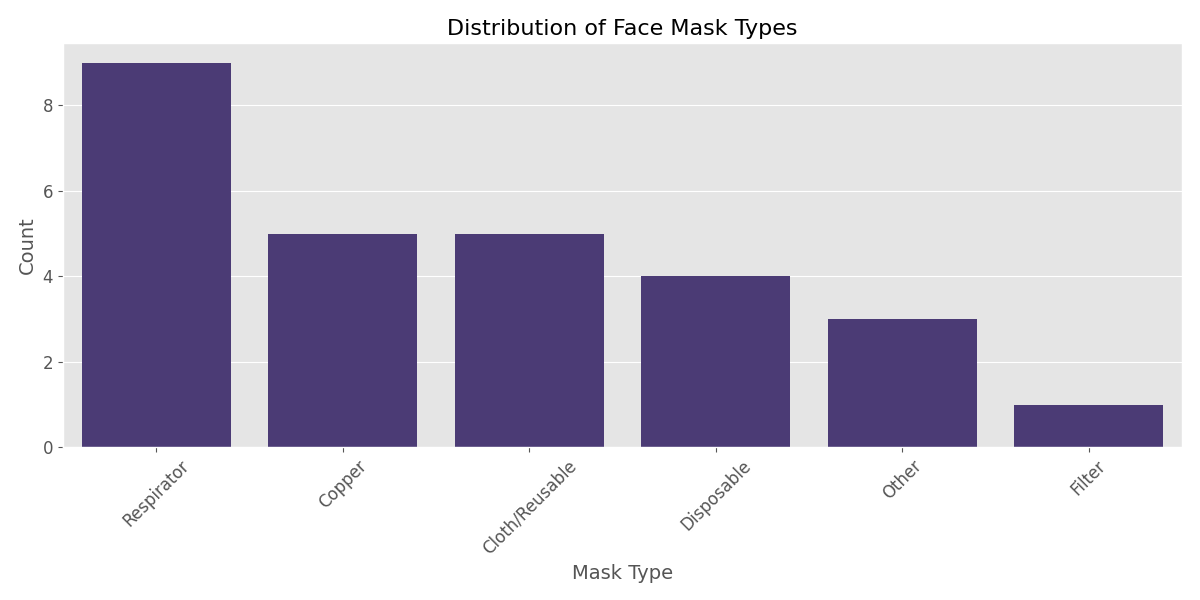
\includegraphics[width=\textwidth]{plots/mask_type_distribution.png}
\end{columns}
\end{frame}

\begin{frame}
\frametitle{Price Positioning by Mask Type}
\begin{columns}
\column{0.45\textwidth}
\begin{itemize}
    \item Significant price variation across mask types
    \item Premium positioning for specialized technologies
    \item Price per mask analysis reveals true value proposition
    \item Opportunity for premium positioning in certain segments
\end{itemize}
\column{0.55\textwidth}
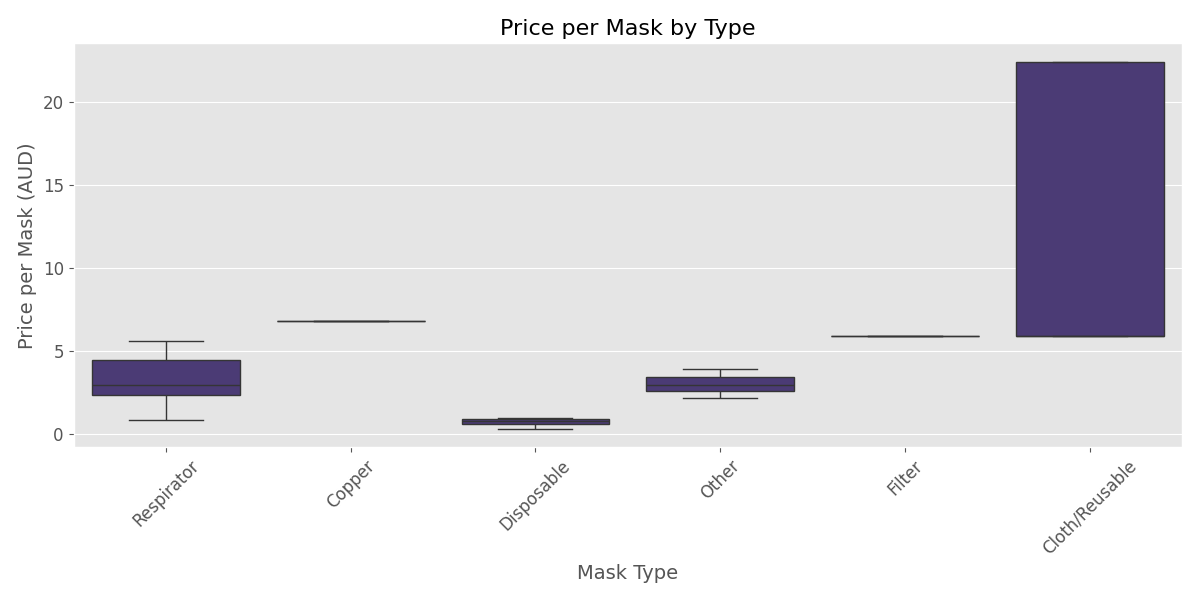
\includegraphics[width=\textwidth]{plots/price_by_mask_type.png}
\end{columns}
\end{frame}

\section{Customer Sentiments}

\begin{frame}
\frametitle{Overall Customer Ratings Distribution}
\begin{columns}
\column{0.45\textwidth}
\begin{itemize}
    \item Strongly polarized ratings distribution
    \item Most products receive either very high or very low ratings
    \item 5-star ratings are most common (50\% of reviews)
    \item Suggests consumers have strong opinions about mask products
\end{itemize}
\column{0.55\textwidth}
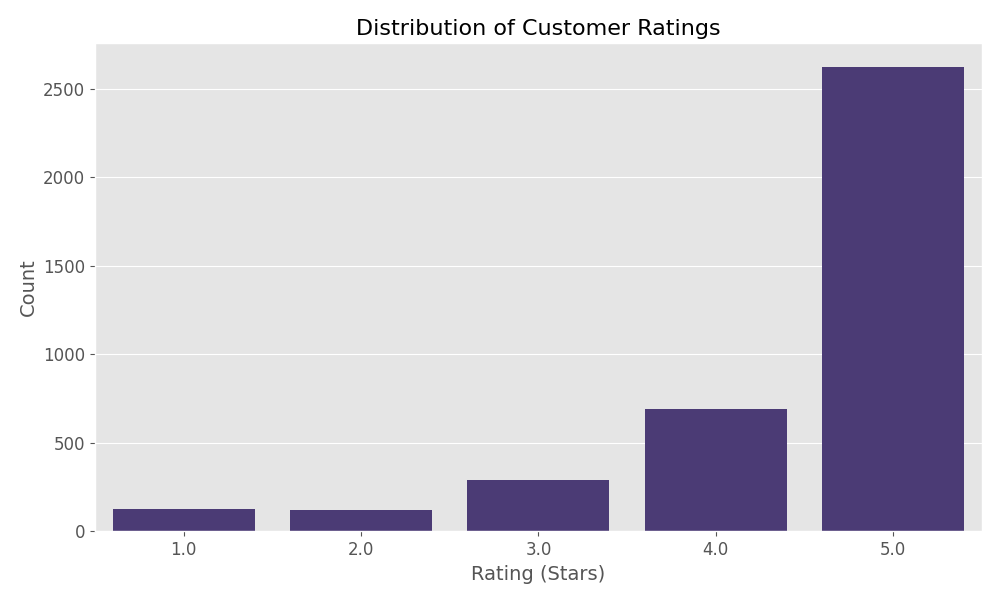
\includegraphics[width=\textwidth]{plots/ratings_distribution.png}
\end{columns}
\end{frame}

\begin{frame}
\frametitle{Sentiment Analysis by Mask Type}
\begin{columns}
\column{0.45\textwidth}
\begin{itemize}
    \item Sentiment scores calculated from review text
    \item Range from -1 (very negative) to +1 (very positive)
    \item Significant variations between mask types
    \item Higher satisfaction with specialized technologies
\end{itemize}
\column{0.55\textwidth}
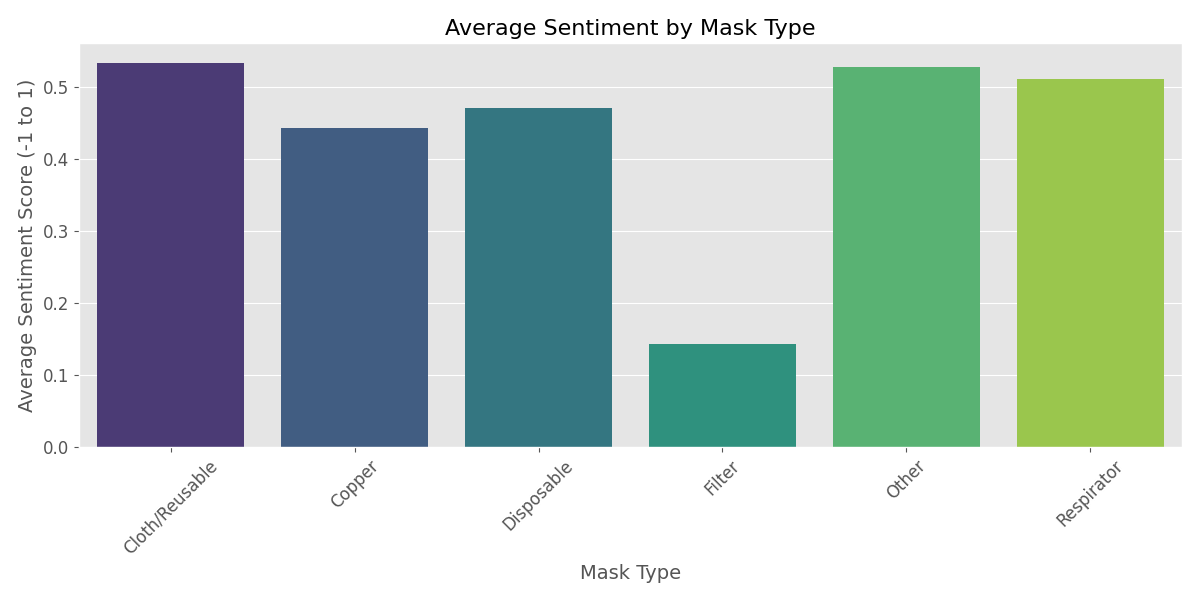
\includegraphics[width=\textwidth]{plots/sentiment_by_mask_type.png}
\end{columns}
\end{frame}

\begin{frame}
\frametitle{Common Themes in Positive Reviews}
\centering
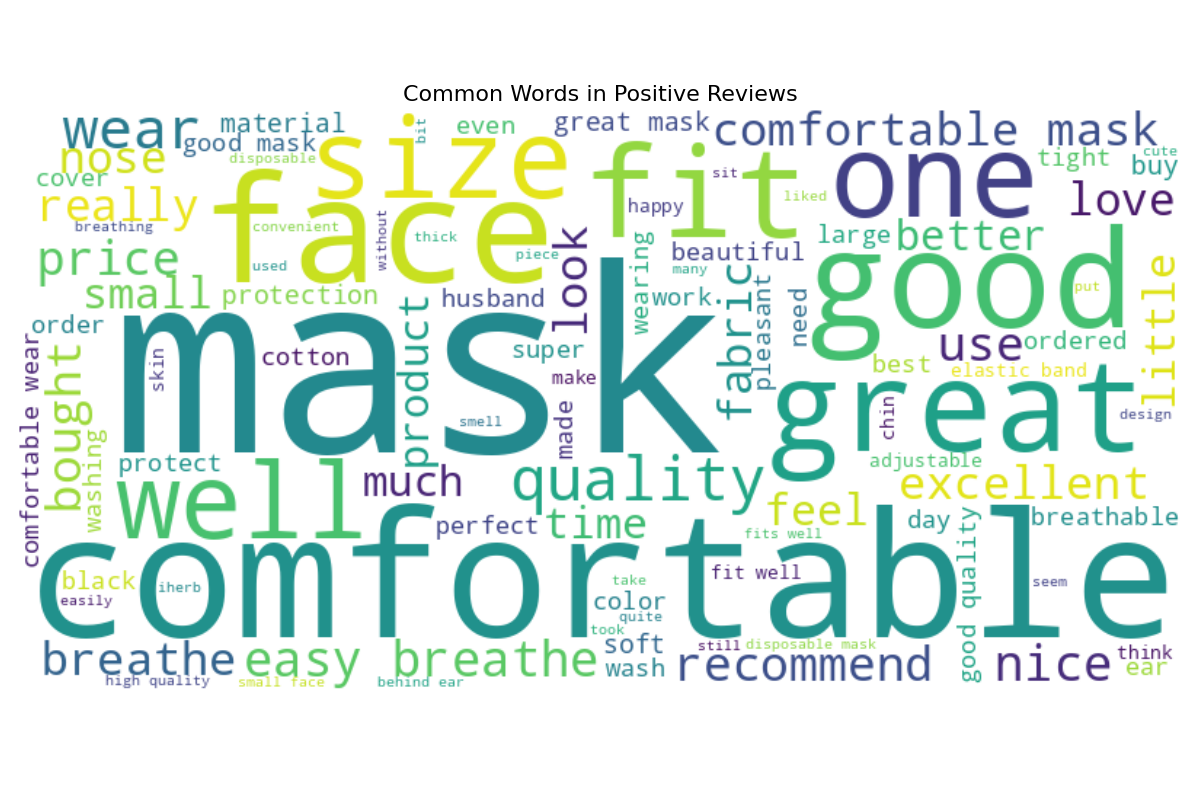
\includegraphics[height=0.8\textheight]{plots/positive_reviews_wordcloud.png}
\end{frame}

\begin{frame}
\frametitle{Common Themes in Negative Reviews}
\centering
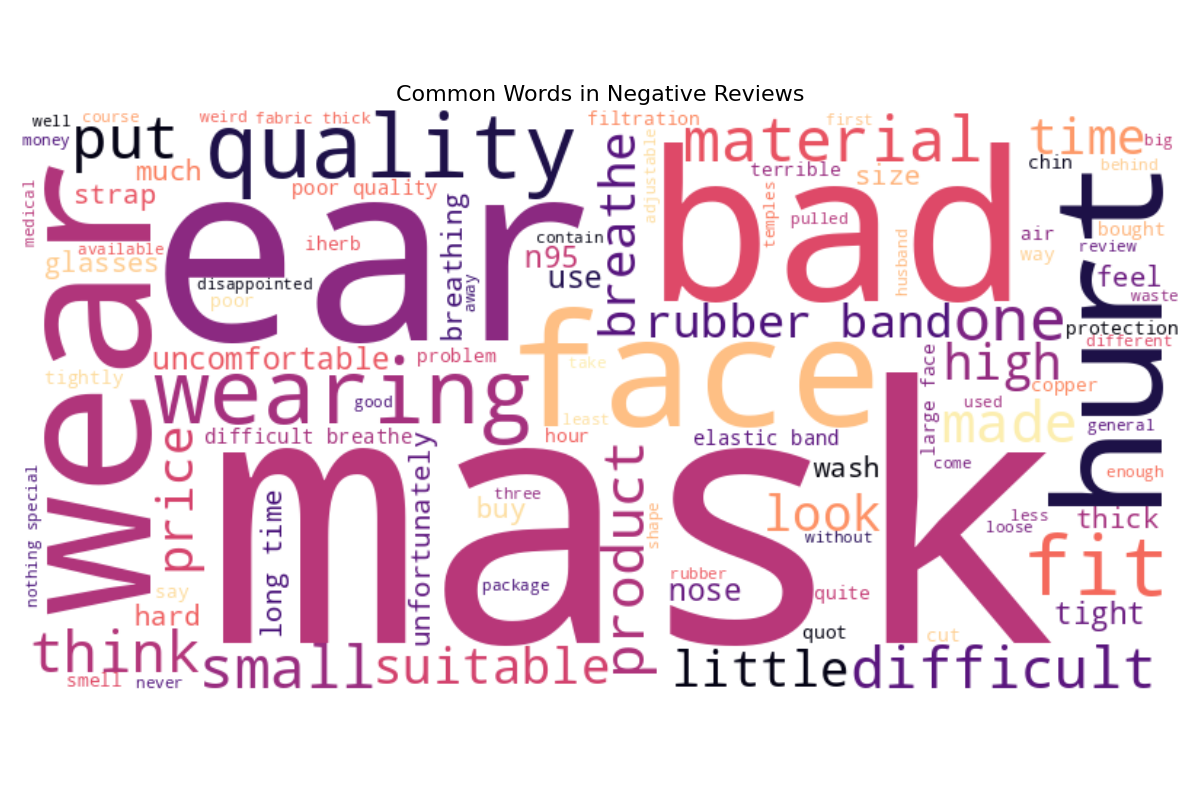
\includegraphics[height=0.8\textheight]{plots/negative_reviews_wordcloud.png}
\end{frame}

\begin{frame}
\frametitle{Most Mentioned Positive Aspects}
\begin{columns}
\column{0.45\textwidth}
\begin{itemize}
    \item Key positive aspects mentioned by satisfied customers
    \item Comfort and fit appear to be primary drivers of satisfaction
    \item Quality is frequently mentioned in positive context
    \item Protection effectiveness is a key positive factor
\end{itemize}
\column{0.55\textwidth}
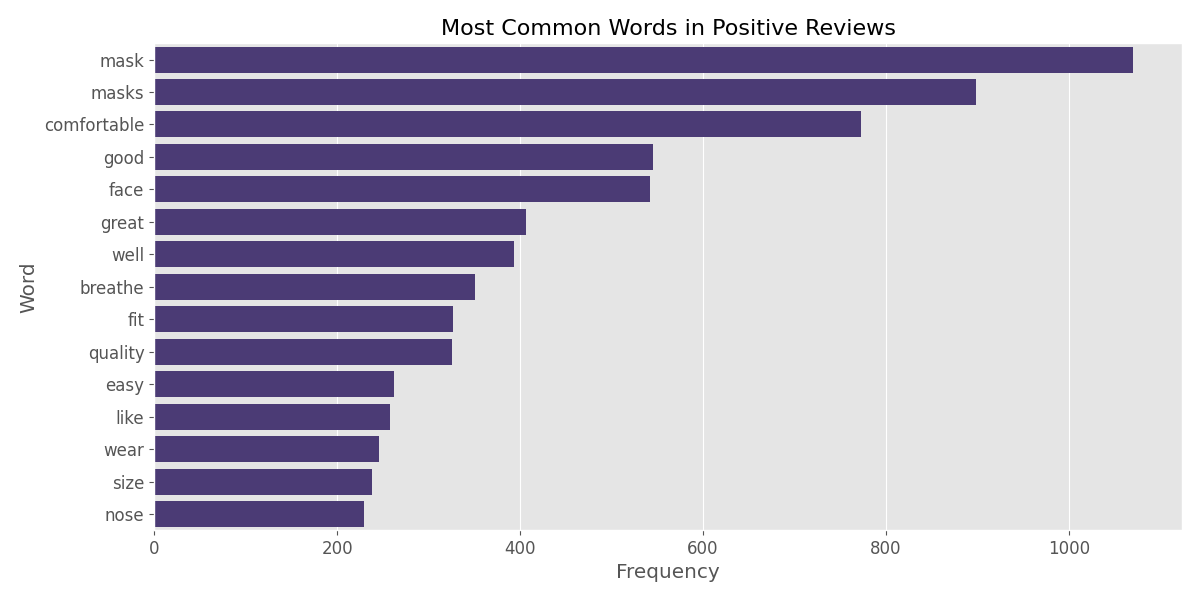
\includegraphics[width=\textwidth]{plots/common_positive_aspects.png}
\end{columns}
\end{frame}

\begin{frame}
\frametitle{Most Mentioned Negative Aspects}
\begin{columns}
\column{0.45\textwidth}
\begin{itemize}
    \item Pain points reported by dissatisfied customers
    \item Sizing and fit issues drive negative sentiments
    \item Quality concerns are frequently mentioned
    \item Issues with ear loops and breathability
\end{itemize}
\column{0.55\textwidth}
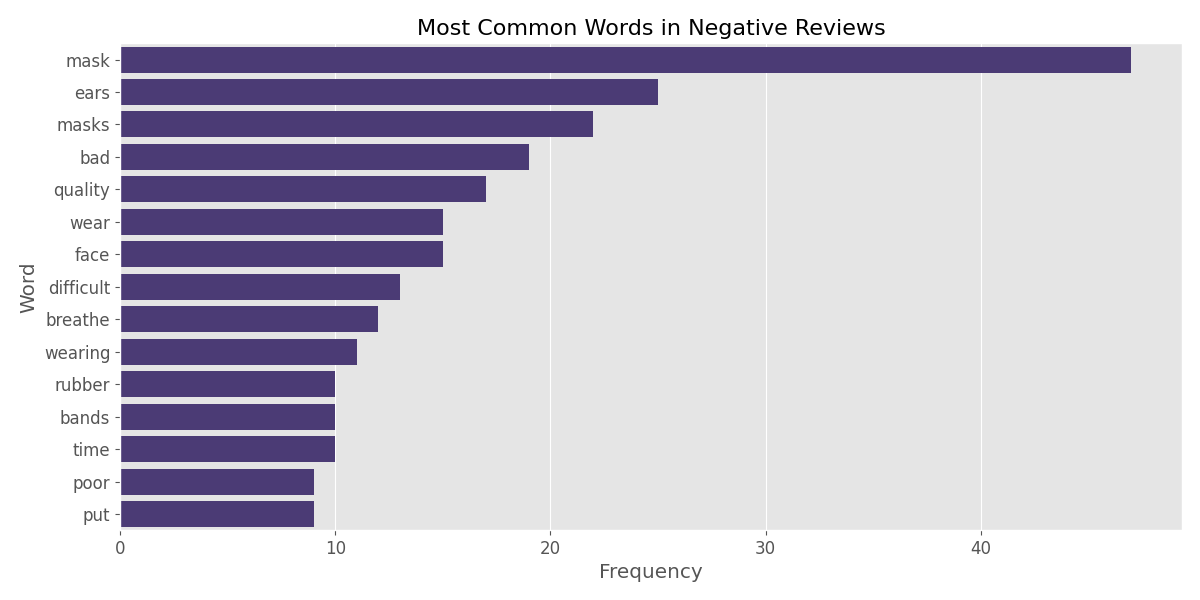
\includegraphics[width=\textwidth]{plots/common_negative_aspects.png}
\end{columns}
\end{frame}

\section{Consumer Segments}

\begin{frame}
\frametitle{Identified Consumer Segments}
\begin{columns}
\column{0.45\textwidth}
\begin{itemize}
    \item Five key consumer segments identified
    \item Segments based on primary concerns in reviews
    \item Fit-focused consumers are largest segment
    \item Protection-focused segment indicates safety concerns
\end{itemize}
\column{0.55\textwidth}
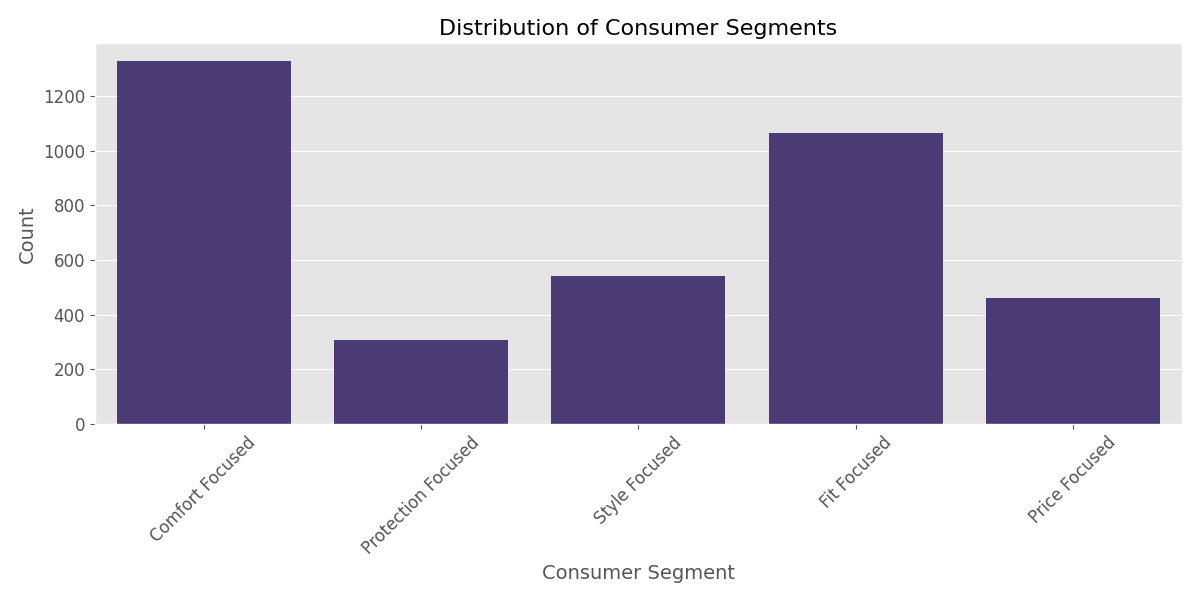
\includegraphics[width=\textwidth]{plots/consumer_segments.png}
\end{columns}
\end{frame}

\begin{frame}
\frametitle{Satisfaction by Consumer Segment}
\begin{columns}
\column{0.45\textwidth}
\begin{itemize}
    \item Average ratings vary across consumer segments
    \item Style-focused consumers show highest satisfaction
    \item Protection-focused consumers are more critical
    \item Comfort-focused consumers' satisfaction varies
\end{itemize}
\column{0.55\textwidth}
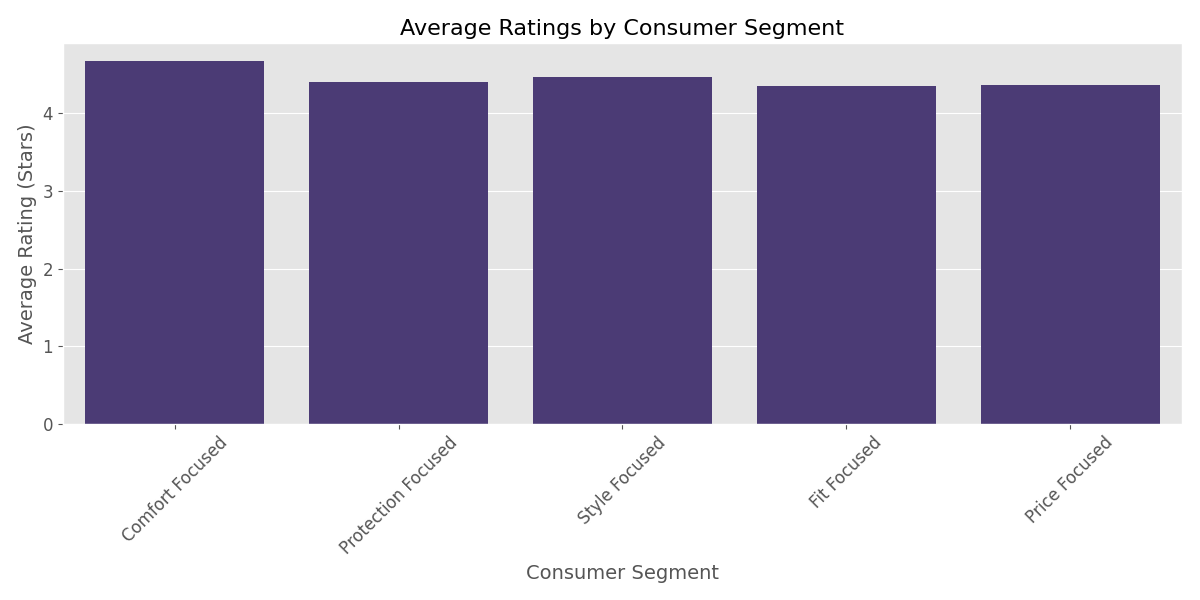
\includegraphics[width=\textwidth]{plots/ratings_by_segment.png}
\end{columns}
\end{frame}

\begin{frame}
\frametitle{Regional Differences in Customer Ratings}
\begin{columns}
\column{0.45\textwidth}
\begin{itemize}
    \item Analysis of ratings by customer language
    \item Significant variations across regions
    \item English-speaking customers most prevalent
    \item Potential for targeted regional marketing
\end{itemize}
\column{0.55\textwidth}
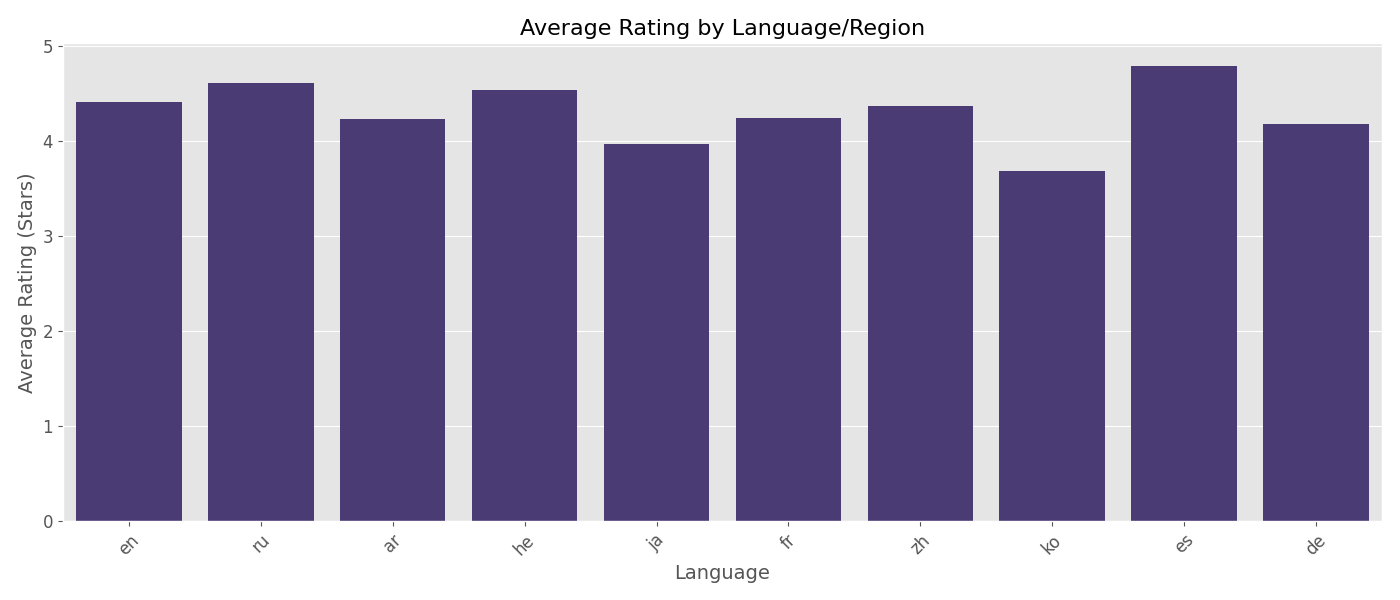
\includegraphics[width=\textwidth]{plots/ratings_by_language.png}
\end{columns}
\end{frame}

\begin{frame}
\frametitle{Sentiment Trends Over Time}
\begin{columns}
\column{0.45\textwidth}
\begin{itemize}
    \item Sentiment score averages by month
    \item Reveals evolution of customer perception
    \item Pandemic-related shifts in expectations
    \item Recent stabilization in sentiment trends
\end{itemize}
\column{0.55\textwidth}
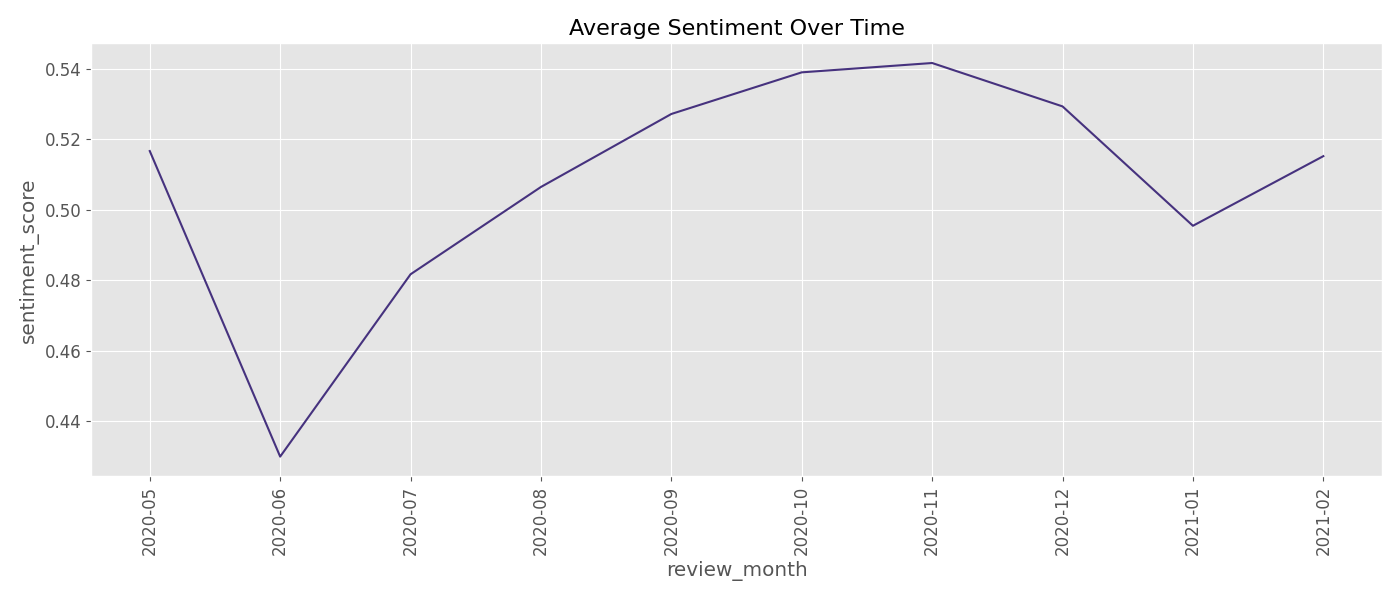
\includegraphics[width=\textwidth]{plots/sentiment_over_time.png}
\end{columns}
\end{frame}

\begin{frame}
\frametitle{Correlation Between Consumer Segments and Ratings}
\centering
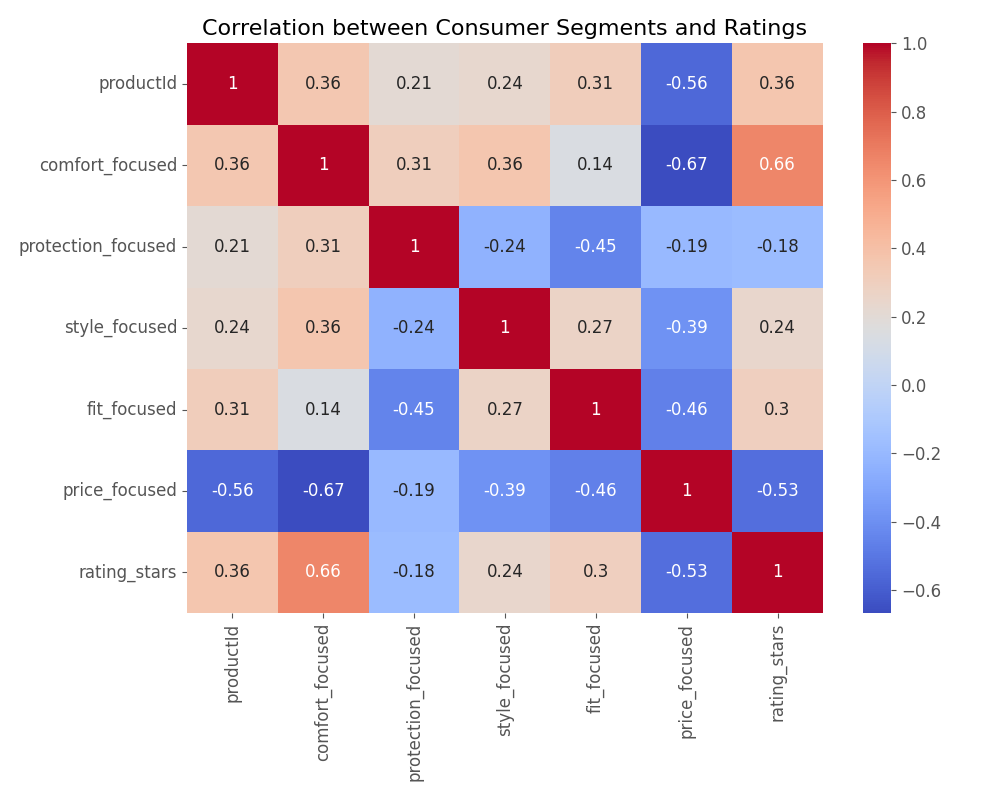
\includegraphics[height=0.8\textheight]{plots/segment_rating_correlation.png}

\small{Correlation analysis reveals which consumer concerns correlate with higher ratings}
\end{frame}

\section{Recommendations}

\begin{frame}
\frametitle{Key Findings \& Strategic Recommendations}
\begin{columns}
\column{0.5\textwidth}
\textbf{Key Findings:}
\begin{itemize}
    \item Fit and comfort are primary drivers of satisfaction
    \item Market is divided between basic and premium segments
    \item Strong polarization in customer sentiment
    \item Technological features command price premiums
\end{itemize}
\column{0.5\textwidth}
\textbf{Strategic Recommendations:}
\begin{itemize}
    \item Focus R\&D on fit improvements
    \item Segment marketing based on identified consumer profiles
    \item Address specific pain points in current products
    \item Explore premium positioning with technological innovations
\end{itemize}
\end{columns}
\end{frame}

\begin{frame}
\frametitle{Product Development Priorities}
\begin{enumerate}
    \item \textbf{Improved Fit Technology:} 
        \begin{itemize}
            \item Develop adjustable designs that accommodate various face shapes
            \item Improve ear loop comfort to address common complaints
        \end{itemize}
    \item \textbf{Breathability Enhancement:} 
        \begin{itemize}
            \item Invest in materials that balance protection with comfort
            \item Focus on reducing heat and moisture buildup
        \end{itemize}
    \item \textbf{Market Segmentation:}
        \begin{itemize}
            \item Develop products targeting specific consumer segments
            \item Create specialized offerings for protection-focused and style-focused consumers
        \end{itemize}
    \item \textbf{Quality Communication:}
        \begin{itemize}
            \item Emphasize quality control in marketing materials
            \item Provide clear information about protection efficacy
        \end{itemize}
\end{enumerate}
\end{frame}

\begin{frame}
\frametitle{Conclusion}
\begin{itemize}
    \item The face mask market shows clear segmentation by product type and consumer preferences
    \item Significant opportunity exists to address current pain points around fit and comfort
    \item Premium positioning is viable with technological innovations
    \item Regional and segment-specific marketing can drive growth
    \item Customer sentiment analysis provides a roadmap for product development
\end{itemize}

\vspace{1cm}
\centering
\Large{Thank you}
\end{frame}

\end{document}